\documentclass{thesis}

\newcommand{\thesistitle}{TODO TITLE}

\usepackage{mathpazo}  % font: palatino vs computer modern
\usepackage{lipsum} % used to fill random text in sections
\usepackage{tikz} % used for sample figure

\newenvironment{dedication}
  {%\clearpage           % we want a new page          %% I commented this
   \thispagestyle{empty}% no header and footer
   \vspace*{\stretch{1}}% some space at the top
   \itshape             % the text is in italics
   \raggedleft          % flush to the right margin
  }
  {\par % end the paragraph
   \vspace{\stretch{3}} % space at bottom is three times that at the top
   \clearpage           % finish off the page
  }

\begin{document}

    % Titlepage (empty pagestyle)
    % Contains titlepage, empty page, "Prodekan + Doktorvater", empty page
    \pagestyle{empty}
    \pagenumbering{gobble}
    %\begin{titlingpage*}
\begin{center}

    Aus dem/der \textit{TODO: institution name} \\

    (Vorstand: \textit{TODO: board members}) \\
    Abteilung \textit{TODO: department} \\
    %\todo{Aktualisieren!}
    (Leiter: \textit{TODO: department head})

    \vfill
    
    %\rule{\linewidth}{0.5mm} \\
    %\vspace*{0.4cm}
    {\Huge \scshape {TODO TITLE \par}} % Title is defined in main.tex
    %\vspace*{0.2cm}
    %\rule{\linewidth}{0.5mm} \\
    %\vspace*{1.6cm}

    \disclosure{TODO: \textit{The format of the dissertation might change in the future, so you should always check that this template is in agreement with the latest version provided by the medical faculty: \textcolor{blue}{\href{https://www.medizinische-fakultaet-hd.uni-heidelberg.de/fakultaet/akademische-laufbahn/promotion/promotion-zum-dr-sc-hum/schreiben-der-dissertation}{Composition Guidelines}}. You should remove this disclosure from the file "titlepage.tex" once you have checked that you are using the correct format.}}

    \vfill

    Inauguraldissertation \\
    zur Erlangung des Doctor scientiarum humanarum (Dr. sc. hum.) \\
    an der \\
    Medizinischen Fakultät Heidelberg \\
    der \\
    Ruprecht-Karls-Universität 

    \vfill

    vorgelegt von \\
    \textit{TODO: name of doctoral candidate} \\
    aus \\
    \textit{TODO: city of birth, and country} \\
    \bigskip
    \textit{TODO: year of submission}

\end{center}

\newpage
\null\newpage
\vspace*{\fill}
 
%\todo{Aktualisieren!}
\noindent Dekan: Prof. Dr. Michael Boutros \\
Doktorvater/Doktormutter: \textit{TODO: name of the official supervisor} 

\newpage
\null\newpage
    \begin{dedication}
\usefont{T1}{LobsterTwo-LF}{bx}{it}
TODO, write here your dedication (one line), or delete the entry in main.tex.
\end{dedication}

    \cleardoublepage
    \tableofcontents
    \cleardoublepage

    \pagestyle{fancy}
    \setcounter{tocdepth}{2}
    \frontmatter
    \setcounter{page}{1}
    % Add acronyms from file (_Acronyms.tex) and add to table of contents
    {
    \chapter*{Acronyms}
    \renewcommand{\leftmark}{ACRONYMS}
    \renewcommand{\rightmark}{ACRONYMS}
    \addcontentsline{toc}{chapter}{Acronyms}
    
    \markboth{Acronyms}{} % Sorgt dafür, dass header für Kapitel Abstract stimmt.(http://www.weinelt.de/latex/markboth.html9
    
    \begin{acronym}[MMMMMMMM]
        \acro{SA}{Sample Acronym}
    \end{acronym}
}

    % Add list of figures and list of tables
    \newpage
    \phantomsection
    \addcontentsline{toc}{chapter}{List of Figures}
    \listoffigures
    \listoftables
    \addcontentsline{toc}{chapter}{List of Tables}

    \mainmatter
    
    
    \mainmatter
    % % Main Body of thesis
    \chapter{Introduction}
\label{chap:introduction}

\lipsum[1]

    \section{Motivation} 
\label{sec:introduction:motivation}

This is an example of a simple acronym that will be included in the list of acronyms: \ac{SA}. These are examples of citations~\cite{smith2020,chen2022,liu2017,miller2020, zhang2016}, this is a second citations\cite{jackson2023,wang2019,nguyen2021,thomas2019,wilson2018}.

This is an example of a figure (Fig.~\ref{fig:motivation:sample_figure}) that is automatically listed in the list of figures:

\begin{figure}[htbp]
    \centering
    \begin{tikzpicture}[scale=1.5]
        \draw[->] (-0.5,0) -- (5,0) node[right] {$x$};
        \draw[->] (0,-1.5) -- (0,1.5) node[above] {$y$};
        \draw[domain=0:4.5, smooth, variable=\x,blue] plot (\x, {sin(\x r)}) node[right] {$f(x) = \sin(x)$};
        \foreach \x in {1,2,3,4}
            \draw (\x cm,1pt) -- (\x cm,-1pt) node[anchor=north] {$\x$};
        \foreach \y in {-1,1}
            \draw (1pt,\y cm) -- (-1pt,\y cm) node[anchor=east] {$\y$};
    \end{tikzpicture}
    \caption{Graph of $y = \sin(x)$.}
    \label{fig:motivation:sample_figure}
\end{figure}

This is an example of a table (Tab.~\ref{tab:motivation:sample_table}) that is automatically included in the list of tables:

\begin{table}[htbp]
    \centering
    \begin{tabular}{|c|c|c|c|c|}
        \hline
        \rowcolor{lightgray}
        Subject ID & Sex & Age & BMI & Comorbidities \\
        \hline
        001 & Male & 25 & 22.5 & None \\
        002 & Female & 30 & 26.8 & Hypertension \\
        003 & Male & 45 & 29.3 & Diabetes \\
        004 & Female & 35 & 23.1 & None \\
        005 & Male & 40 & 27.6 & Hyperlipidemia \\
        \hline
    \end{tabular}
    \caption{Sample table with random values.}
    \label{tab:motivation:sample_table}
\end{table}

\disclosure{Important disclosure}{This is an example of a "disclosure" that can be used to disclose relevant information or highlight important text.}

\researchquestion{1}{This an example of a research question box, that can be used to highlight the statements of your research questions.}

    \section{Background} 
\label{sec:introduction:background}

\lipsum[1-3]
    \section{Related Work} 
\label{sec:introduction:related_work}


\lipsum[1-3]
    \section{Objectives and Contributions}
\label{sec:introduction:objectives}


\lipsum[1-3]

    \section{Outline} 
\label{sec:introduction:outline}


\lipsum[1-3]
        
    \chapter{Materials and Methodology}
\label{chap:materials_and_methods}

\lipsum[1]   

    \section{TODO TITLE} 
\label{sec:methods:methods_one}

\lipsum[1-3]
    
    \chapter{Results}
\label{chap:results}

\lipsum[1]

    \section{TODO TITLE}
\label{sec:results:results_one}

\lipsum[1-3]
    \chapter{Discussion}
\label{chap:discussion}

\lipsum[1]   

    \section{TODO TITLE} 
\label{sec:discussion:diss_one}

\lipsum[1-3]

    \chapter{Summary}


\lipsum[1-5]
    \chapter{Zusammenfassung}

\lipsum[1-5]
    
    \clearpage
    \phantomsection
    \addcontentsline{toc}{chapter}{Bibliography}
    \markboth{Bibliography}{Bibliography}
    \bibliography{refs} % In overleaf you can link to Zotero. Go to "new file"->"From Zotero"

    \chapter*{Own Contributions}
\addcontentsline{toc}{chapter}{Own Contributions and Publications}
\markboth{Own Contributions and Publications}{Own Contributions and Publications}
\label{chap:contributions}

This chapter gives an overview of my contributions in distinction to team efforts.


\section*{Own share in data acquisition and data analysis}
\phantomsection
\addcontentsline{toc}{section}{Own share in data acquisition and data analysis}
\label{sec:own-data-acquisition}

    
\lipsum[1]

\paragraph{Own share in Data Acquisition.}
\lipsum[1]  

\paragraph{Own share in Data Analysis.}
\lipsum[1] 
        
        

\section*{Own Publications}
\addcontentsline{toc}{section}{Own Publications}
\label{sec:own-publications}

In this section, all publications that I was a part of and contributed to during my Ph.D. work are listed. It is subdivided into \textit{First Authorships} and \textit{Co-Authorships}.
\hfill \break

\subsection*{First Authorships - Peer Reviewed International Journal Publications} \label{sec:publications:peer_reviewed_journal_first}

\begin{itemize}
    \item[] \textbf{J. Smith}, A. Johnson, R. Martinez, C. Lee, S. Wang. \textbf{Journal of Advanced Robotics}. \textit{Enhancing grasping capabilities of robotic hands using tactile sensors}. \url{doi:10.1234/JAR.567890}.
\end{itemize}

\subsection*{First Authorships - Peer Reviewed International Conference Publications} \label{sec:publications:peer_reviewed_conf_first}

\begin{itemize}
    \item[] \textbf{J. Smith}, A. Johnson, R. Martinez, C. Lee, S. Wang. \textbf{Journal of Advanced Robotics}. \textit{Enhancing grasping capabilities of robotic hands using tactile sensors}. \url{doi:10.1234/JAR.567890}.
\end{itemize}

\subsection*{Co-Authorships} \label{sec:publications:other_co}

\begin{itemize}
    \item[] \textbf{J. Smith}, A. Johnson, R. Martinez, C. Lee, S. Wang. \textbf{Journal of Advanced Robotics}. \textit{Enhancing grasping capabilities of robotic hands using tactile sensors}. \url{doi:10.1234/JAR.567890}.
\end{itemize}


    \pagestyle{plain}
    % Include CV from PDF like this:
    \phantomsection
    \addcontentsline{toc}{chapter}{Curriculum Vitae}
    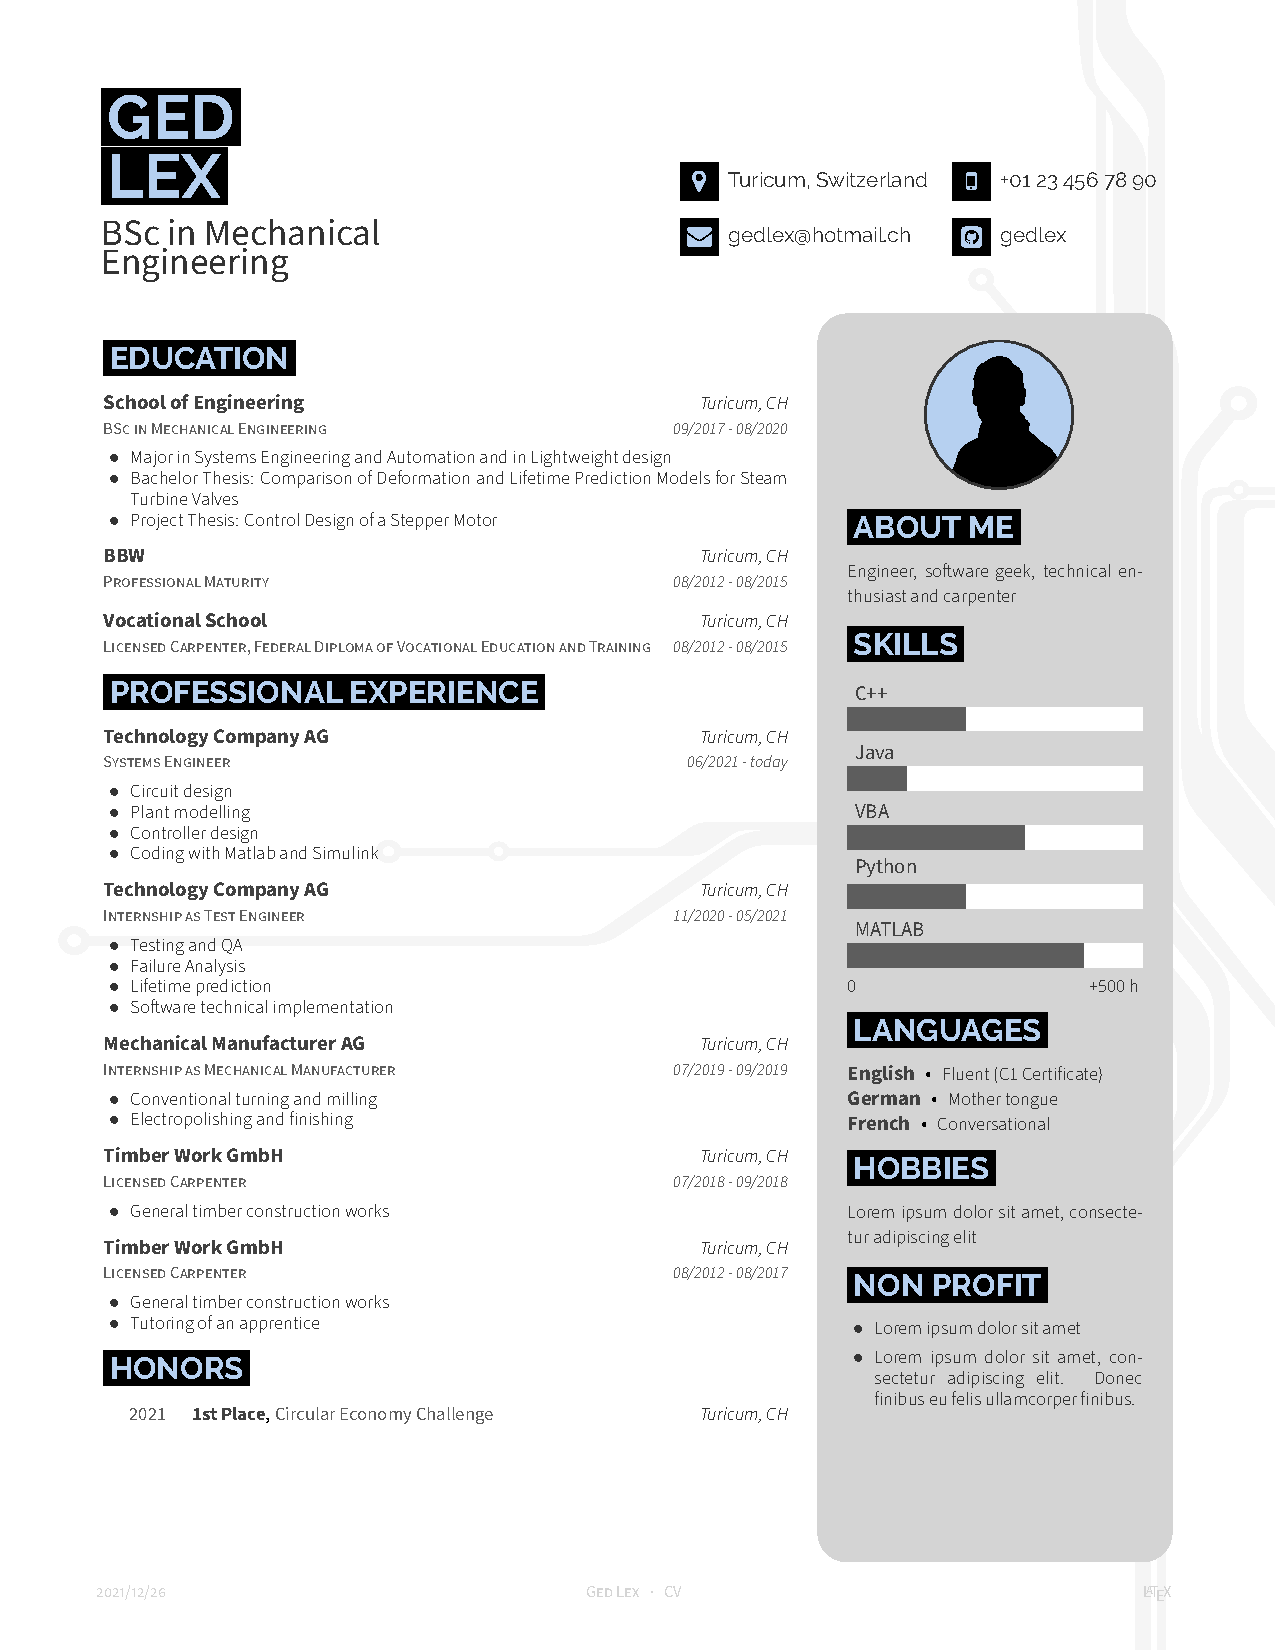
\includepdf[pages=-,frame,scale=.77,pagecommand={\thispagestyle{plain}}]{figures/CV.pdf}
    

    \chapter*{Appendix}
\addcontentsline{toc}{chapter}{Appendix}

\lipsum[1-3]
    \chapter*{Acknowledgement}
\addcontentsline{toc}{chapter}{Acknowledgement}

\lipsum[1-3]

    \chapter*{Eidesstattliche Versicherung}
\vspace{-6em}{\Huge\color{dkfzgray2} Statutory Declaration}
\addcontentsline{toc}{chapter}{Eidesstattliche Versicherung (Affidavit) in German}
    
    \begin{enumerate}
        \setlength{\itemsep}{0pt}
        \item Bei der eingereichten Dissertation zu dem Thema \emph{\textbf{\thesistitle}} handelt es sich um meine eigenständig erbrachte Leistung.\\
        \emph{\small\color{dkfzgray2} I herewith formally declare that I have written the submitted dissertation \textbf{\thesistitle} independently.}
        
        \item Ich habe nur die angegebenen Quellen und Hilfsmittel benutzt und mich keiner unzulässigen Hilfe Dritter bedient. Insbesondere habe ich wörtlich oder sinngemäß aus anderen Werken übernommene Inhalte als solche kenntlich gemacht.\\
        \emph{\small\color{dkfzgray2}  I did not use any third party support except for the quoted literature and other sources mentioned in the text. Content from other work, either literally or in content, has been declared as such.}
        
        \item Die Arbeit oder Teile davon habe ich bislang nicht an einer Hochschule des In- oder Auslands als Bestandteil einer Prüfungs- oder Qualifikationsleistung vorgelegt.\\
        \emph{\small\color{dkfzgray2} The thesis has not been submitted to any examination body in this, or similar, form. }
        
        \item Die Richtigkeit der vorstehenden Erklärungen bestätige ich.\\
        \emph{\small\color{dkfzgray2} I confirm the correctness of the aforementioned declarations.}
        
        \item Die Bedeutung der eidesstattlichen Versicherung und die strafrechtlichen Folgen einer unrichtigen oder unvollständigen eidesstattlichen Versicherung sind mir bekannt. Ich versichere an Eides statt, dass ich nach bestem Wissen die reine Wahrheit erklärt und nichts verschwiegen habe.\\
        \emph{\small\color{dkfzgray2} I am aware of the legal consequences of this declaration. To the best of my knowledge I have told the pure truth and not concealed anything.}
    \end{enumerate}
    
    \begin{tabular}{p{3cm}p{5cm}p{4cm}}
          &  & \\
          & & \\
          &Heidelberg, \today & \hrulefill\\
          & & \textit{TODO: name of doctoral student}
    \end{tabular}
    \chapter*{Angabe zu verwendeten KI-basierter Elektronischer Hilfsmittel}
\vspace{-6em}{\Huge\color{dkfzgray2} Information on the use of AI-based tools}
\addcontentsline{toc}{chapter}{Angabe zu verwendeten KI-basierter Elektronischer Hilfsmittel}

Zur Dokumentation der verwendeten Hilfsmittel ist der schriftlichen Ausarbeitung ein besonderer Anhang hinzugefügt, der eine Liste und Beschreibung aller verwendeter KI-basierter Hilfsmittel enthält. Der besondere Anhang zur Dokumentation der verwendeten Hilfsmittel erfüllt folgende Kriterien:

\emph{\small\color{dkfzgray2} To document the tools used, a special appendix has been added to the written report, which contains a list and description of all AI-based tools used. The special appendix to document the tools used meets the following criteria:}

\begin{enumerate}
    \item Auflistung der Ziele, für die die KI-basierten Hilfsmittel in der vorliegenden Arbeit eingesetzt wurden.\\
    \emph{\small\color{dkfzgray2} List of the goals for which the AI-based tools were used in this work.}
    \item Dokumentation der Verwendungsweise der KI-basierten Hilfsmittel.\\
    \emph{\small\color{dkfzgray2} Documentation of how AI-based tools are used.}
    \item Nennung der Kapitel und Abschnitte der vorliegenden Arbeit, in denen die KI-basierten Hilfsmittel eingesetzt wurden, um Inhalte zu erzeugen.\\
    \emph{\small\color{dkfzgray2} Identification of the chapters and sections of this work in which AI-based tools were used to generate content.}
\end{enumerate}

Der Gebrauch dieser Hilfsmittel inklusive Art, Ziel und Umfang des Gebrauchs wurde mit meinem offiziellen Betreuer / meiner offiziellen Betreuerin \textbf{TODO NAME OF SUPERVISOR} abgesprochen.

\emph{\small\color{dkfzgray2} The use of these aids, including the type, purpose and extent of use, has been agreed with my official supervisor \textbf{TODO NAME OF SUPERVISOR}.}
\newpage
Mir ist bewusst, dass insbesondere der Versuch einer nicht dokumentierten Nutzung KI- basierter Hilfsmittel als Täuschungsversuch zu werten ist:

\emph{\small\color{dkfzgray2} I am aware that in particular the attempt to use AI-based tools without documentation is to be regarded as an attempt at deception:}

Gem. § 16 Abs. 2 der Promotionsordnung „Dr. med. / dent.“:
„Ergibt sich vor Aushändigung der Promotionsurkunde, dass der Kandidat/die Kandidatin bei einer Promotionsleistung getäuscht hat, so können einzelne oder alle Promotionsleistungen für ungültig erklärt werden. In schweren Fällen kann die Zulassung zum Promotionsverfahren zurückgenommen werden.“

\emph{\small\color{dkfzgray2} According to § 16 paragraph 2 of the doctoral regulations for "Dr. med. / dent.":
"If it emerges before the doctoral certificate is issued that the candidate has cheated in a doctoral achievement, individual or all doctoral achievements can be declared invalid. In serious cases, admission to the doctoral process can be withdrawn.}

Und § 16 Abs. 2 der Promotionsordnung „Dr. sc. hum.“:
„Ergibt sich vor Aushändigung der Promotionsurkunde, dass der Doktorand / Doktorandin bei einer Promotionsleistung getäuscht hat, so kann der Promotionsausschuss diese Promotionsleistung oder alle bisher erbrachten Promotionsleistungen für ungültig erklären. In besonders schweren Fällen kann der Promotionsausschuss die Annahme als Doktorand / Doktorandin endgültig widerrufen.“

\emph{\small\color{dkfzgray2} And § 16 paragraph 2 of the doctoral regulations “Dr. sc. hum.”:
“If it emerges before the doctoral certificate is issued that the doctoral candidate has cheated in a doctoral achievement, the doctoral committee can declare this doctoral achievement or all doctoral achievements to date invalid. In particularly serious cases, the doctoral committee can permanently revoke the acceptance as a doctoral candidate.”}

\begin{tabular}{p{3cm}p{5cm}p{4cm}}
      &  & \\
      & & \\
      &Heidelberg, \today & \hrulefill\\
      & & \textit{TODO: name of doctoral student}
\end{tabular}

    \chapter*{Anhang: Verwendete KI-basierte elektronische Hilfsmittel}
\vspace{-6em}{\Huge\color{dkfzgray2} Appendix: AI-based tools used}
\addcontentsline{toc}{chapter}{Anhang: Verwendete KI-basierte elektronische Hilfsmittel}

Im Folgenden werden die im Rahmen dieser Dissertation verwendeten KI-basierten
Hilfsmittel gemäß den Vorgaben aus dem Anhang „Angabe zu verwendeten KI-basierten
elektronischen Hilfsmitteln" dokumentiert.

\emph{\small\color{dkfzgray2} The AI-based tools used in the course of this
dissertation are documented below, in accordance with the requirements set out
in the appendix ``Information on the use of AI-based tools''.}

\bigskip

% ---------------------------------------------------------------------------
% ANLEITUNG (vor Einreichung löschen):
%
% Für JEDES verwendete KI-Tool (z. B. Claude / Claude Code, ChatGPT, DeepL,
% Grammarly, GitHub Copilot, ...) einen eigenen Block nach untenstehendem
% Muster anlegen. Pflichtangaben laut KI-Leitlinie der Universität Heidelberg:
%   1. Ziel:              Wofür wurde das Tool eingesetzt?
%   2. Verwendungsweise:  Wie genau wurde es eingesetzt? (z. B. Grammatik-
%                         korrektur, Übersetzung, Textentwurf, Code-Erstellung,
%                         Literaturrecherche) UND die Bestätigung, dass jeder
%                         Output eigenständig fachlich geprüft wurde.
%   3. Betroffene Kapitel/Abschnitte: konkret benennen, nicht "überall".
%
% Wurde gar keine KI verwendet, hier explizit "Es wurden keine KI-basierten
% Hilfsmittel verwendet." eintragen statt das Kapitel leer zu lassen.
% ---------------------------------------------------------------------------

\section*{TODO: Name des Tools (z.\,B. Claude Code)}
\addcontentsline{toc}{section}{TODO: Name des Tools}

\begin{enumerate}
    \item \textbf{Ziel.} TODO: Wofür wurde das Tool eingesetzt (z.\,B.
    Rechtschreib-/Grammatikprüfung, Literaturrecherche, Umformulierung
    bestehenden Textes, Erstellung von Textentwürfen, Code-Generierung für
    Abbildungen, Konvertierung eines bestehenden Entwurfs in dieses
    LaTeX-Template)?\\
    \emph{\small\color{dkfzgray2} Goal. TODO: What was the tool used for?}

    \item \textbf{Verwendungsweise.} TODO: Wie wurde das Tool konkret
    eingesetzt? Wichtig: hier auch festhalten, dass alle Vorschläge/Entwürfe
    vom Verfasser/von der Verfasserin eigenständig fachlich geprüft, korrigiert
    und erst danach übernommen wurden.\\
    \emph{\small\color{dkfzgray2} How used. TODO: How exactly was the tool
    used? State that all suggestions/drafts were independently reviewed,
    corrected, and approved by the author before adoption.}

    \item \textbf{Betroffene Kapitel/Abschnitte.} TODO: Konkrete Kapitel/
    Abschnitte benennen (z.\,B. "Einleitung, Abschnitt 2.3, Abbildungen 3.4
    und 3.7").\\
    \emph{\small\color{dkfzgray2} Chapters/sections affected. TODO: Name the
    specific chapters/sections.}
\end{enumerate}

\bigskip
\textit{TODO: diesen Block für jedes weitere verwendete KI-Tool duplizieren.}


\end{document}
